\begin{figure}[H]
    \centering
    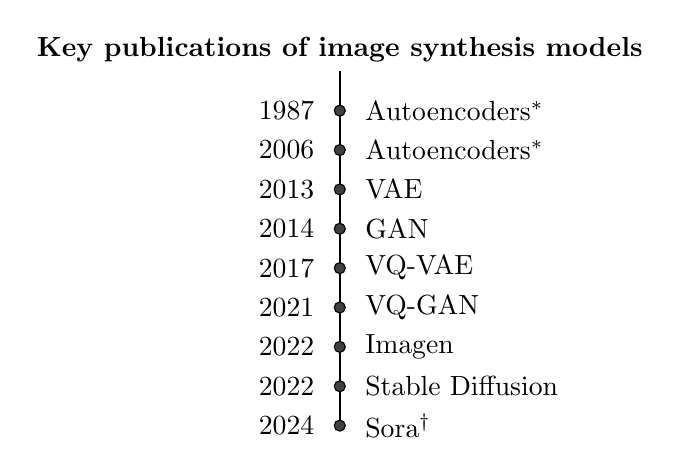
\begin{tikzpicture}
        \def\step{0.5} % step size for vertical spacing
        \def\numtimeline{9} % Number of events in the timeline

        % Define timeline line
        \draw[thick, color=black] (0,0) -- (0,-\numtimeline*\step);

        % Define timeline events with adjusted positions
        \foreach \i/\year/\text in 
        {
            1/1987/Autoencoders$^*$, 
            2/2006/Autoencoders$^*$, 
            3/2013/VAE, 
            4/2014/GAN, 
            5/2017/VQ-VAE,
            6/2021/VQ-GAN,
            7/2022/Imagen,
            8/2022/Stable Diffusion,
            9/2024/Sora$^\dag$
        } {
        \draw[fill=darkgray] (0,-\i*\step) circle (2pt);
        \node[anchor=east] at (-0.2,-\i*\step) {\year};
        \node[anchor=west] at (0.2,-\i*\step) {\text};
        }

        % Define timeline title
        \node[anchor=south] at (0,0) {\textbf{Key publications of image synthesis models}};
    \end{tikzpicture}
    \caption{Chronology of key image generation models publications $^*$The earliest mention of autoencoders appears in an 1986 publication \cite{autoencoder_original_paper_1986}, however the model was not widely used until 2006 when Hinton published a paper that uses autoencoders for dimensionality reduction \cite{autoencoder_2006_paper} which sparked interest in the model again.$^\dag$Although Sora \cite{sora_website} is not specifically an image generation model, it is considered a significant advancement in video synthesis field, which largely relies on image generation.}
    \label{fig:timeline}
  \end{figure}